\documentclass{beamer}

\usetheme{Warsaw}
\setbeamertemplate{footline}[frame number]
\usepackage[french]{babel}
\usepackage{hyperref}
\usepackage[utf8]{inputenc}
\usepackage[version=0.96]{pgf}
\usepackage{tikz}
\usetikzlibrary{arrows, positioning}


\title{A2C}
\author{Team MALT : \\
  Lucien Boillod \\
  Maxime Gaudron \\
  Thibaud Michaud \\
Charles Yaiche }

\AtBeginSection[]
{
  \begin{frame}<beamer>
    \tableofcontents[
      currentsection,
      sectionstyle=show/shaded,
      subsectionstyle=show/shaded/hide
    ]
  \end{frame}
}

\AtBeginSubsection[]
{
  \begin{frame}<beamer>
    \tableofcontents[
      currentsection,
      sectionstyle=show/shaded,
      subsectionstyle=show/shaded/hide
    ]
  \end{frame}
}

\begin{document}
\maketitle

\begin{frame}
  \tableofcontents
\end{frame}

\begin{frame}
  \begin{center}
    La team MALT (anciennement Ghom) \\
    vous présente le projet A2C
  \end{center}
\end{frame}
\section{lexeur/parseur}
\begin{frame}
  \begin{center}
    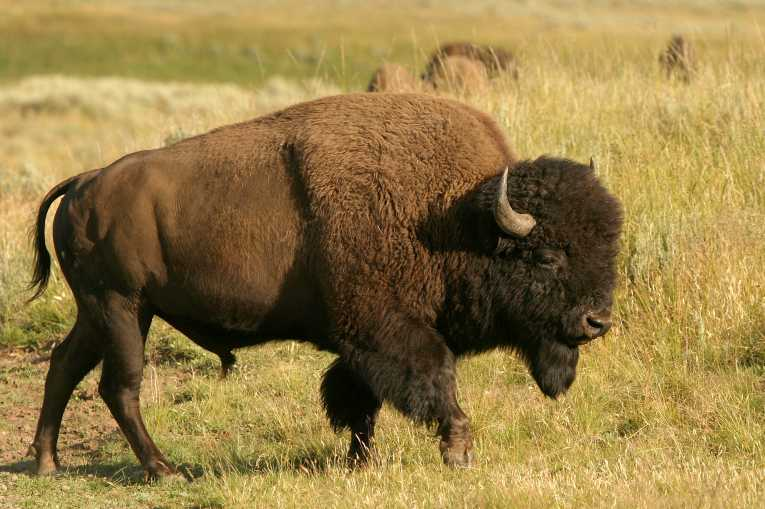
\includegraphics[scale=0.3]{bison.jpg}
  \end{center}
\end{frame}
\section{AST}
\begin{frame}
\begin{center}
\begin{tikzpicture}[->,>=stealth',shorten >=1pt,auto,node distance=2cm, thick,main node/.style={fill=blue!20,draw,font=\sffamily}]
  %
    \node[main node] (6) {instruction (assignation)};
    \node[main node] (7) [below left of=6]{identifiant (a)};
    \node[main node] (1) [below right of=6]{expression (*)};
    \node[main node] (2) [below left of=1] {expression (2)};
    \node[main node] (3) [below right of=1] {expression (+)};
    \node[main node] (4) [below left of=3] {expression (20)};
    \node[main node] (5) [below right of=3] {expression (1)};
    \path[every node/.style={font=\sffamily\small}]
    (1) edge node {} (2)
    (1) edge node {} (3)
    (3) edge node {} (4)
    (3) edge node {} (5)
    (6) edge node {} (7)
    (6) edge node {} (1)
    ;
\end{tikzpicture}
\end{center}
\end{frame}

\section{génération de code}
\begin{frame}
\begin{center}
\begin{tikzpicture}[->,>=stealth',shorten >=1pt,auto,node distance=2cm, thick,main node/.style={fill=blue!20,draw,font=\sffamily}]
  %
    \node[main node] (6) {instruction (assignation)};
    \node[main node] (7) [below left of=6]{identifiant (a)};
    \node[main node] (1) [below right of=6]{expression (*)};
    \node[main node] (2) [below left of=1] {expression (2)};
    \node[main node] (3) [below right of=1] {expression (+)};
    \node[main node] (4) [below left of=3] {expression (20)};
    \node[main node] (5) [below right of=3] {expression (1)};
    \path[every node/.style={font=\sffamily\small}]
    (1) edge node {} (2)
    (1) edge node {} (3)
    (3) edge node {} (4)
    (3) edge node {} (5)
    (6) edge node {} (7)
    (6) edge node {} (1)
    ;
\end{tikzpicture}
\\\vspace{0.5cm}\textbf{a = (2 * ( 20 + 1));}
\end{center}
\end{frame}

\section{analyse semantique}
\begin{frame}
\begin{center}
\begin{tikzpicture}[->,>=stealth',shorten >=1pt,auto,node distance=2cm, thick,main node/.style={fill=blue!20,draw,font=\sffamily}]
  %
    \node[main node] (6) {instruction (assignation)};
    \node[main node] (7) [below left of=6]{identifiant (a)};
    \node[main node] (1) [below right of=6]{expression (*)};
    \node[main node] (2) [below left of=1] {type INT : 2};
    \node[main node] (3) [below right of=1] {expression (+)};
    \node[main node] (4) [below left of=3] {type INT : 20};
    \node[main node] (5) [below right of=3] {type INT : 1};
    \path[every node/.style={font=\sffamily\small}]
    (1) edge node {} (2)
    (1) edge node {} (3)
    (3) edge node {} (4)
    (3) edge node {} (5)
    (6) edge node {} (7)
    (6) edge node {} (1)
    ;
\end{tikzpicture}
\\\vspace{0.5cm}\textbf{a = (2 * ( 20 + 1));}
\end{center}
\end{frame}
\begin{frame}
\begin{center}
\begin{tikzpicture}[->,>=stealth',shorten >=1pt,auto,node distance=2cm, thick,main node/.style={fill=blue!20,draw,font=\sffamily}]
  %
    \node[main node] (6) {instruction (assignation)};
    \node[main node] (7) [below left of=6]{identifiant (a)};
    \node[main node] (1) [below right of=6]{expression (*)};
    \node[main node] (2) [below left of=1] {type INT : 2};
    \node[main node] (3) [below right of=1] {expression (+)};
    \node[main node] (4) [below left of=3] {type INT : 20};
    \node[main node] (5) [below right of=3] {type BOOL : vrai};
    \path[every node/.style={font=\sffamily\small}] 
    (1) edge node {} (2)
    (1) edge node {} (3)
    (3) edge node {} (4)
    (3) edge node {} (5)
    (6) edge node {} (7)
    (6) edge node {} (1)
    ;
\end{tikzpicture}
\\\vspace{0.5cm}\textbf{a = (2 * ( 20 + 1));}
\end{center}
\end{frame}
\section{Site web}
\begin{frame}
\begin{center}
\url{http://a2c.lucien-boillod.net/}
\end{center}
\end{frame}
\section{Conclusion}


\begin{frame}
  \begin{center}
    \Large{Questions?}\\
  \end{center}
\end{frame}

\end{document}
